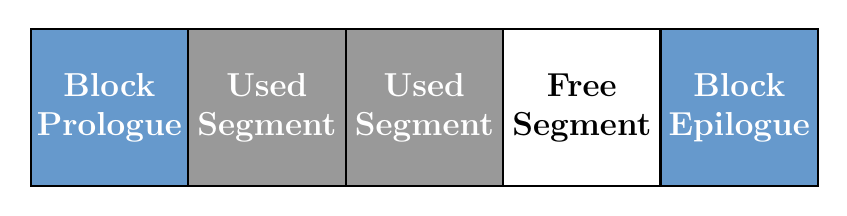
\begin{tikzpicture}

% Define colors
\definecolor{prologue}{rgb}{0.4, 0.6, 0.8}
\definecolor{used}{rgb}{0.6, 0.6, 0.6}
\definecolor{free}{rgb}{1, 1, 1}

% Draw the blocks
\fill[prologue] (0,0) rectangle (2,2);
\node[align=center, text=white, font=\bfseries\large] at (1, 1) {Block\\Prologue};

\fill[used] (2,0) rectangle (4,2);
\node[align=center, text=white, font=\bfseries\large] at (3, 1) {Used\\Segment};

\fill[used] (4,0) rectangle (6,2);
\node[align=center, text=white, font=\bfseries\large] at (5, 1) {Used\\Segment};

\fill[free] (6,0) rectangle (8,2);
\node[align=center, text=black, font=\bfseries\large] at (7, 1) {Free\\Segment};

\fill[prologue] (8,0) rectangle (10,2);
\node[align=center, text=white, font=\bfseries\large] at (9, 1) {Block\\Epilogue};

% Draw the borders
\draw[thick] (0,0) rectangle (2,2);
\draw[thick] (2,0) rectangle (4,2);
\draw[thick] (4,0) rectangle (6,2);
\draw[thick] (6,0) rectangle (8,2);
\draw[thick] (8,0) rectangle (10,2);

\end{tikzpicture}
